\documentclass{article}
\usepackage{SRM2}
\usepackage{graphicx}
\usepackage{url}
\usepackage{color}

\title{The AviaNZ Bioacoustic Analysis Software (v 3.0)}
\author{The AviaNZ Team \\(\url{stephen.marsland@vuw.ac.nz})}
\date{September 2020}

%\usepackage[usenames, dvipsnames]{color}

%Revise with track changes
\usepackage{soulutf8}
\usepackage[normalem]{ulem}
\usepackage{multirow}
\usepackage{booktabs}

\begin{document}
\maketitle

This is the user manual for version 3.0 of the AviaNZ program. There are several changes to this version of the program, of which the most obvious are (i) improved species filters, including the ability to train your own, and (ii) the ability to process bat recordings from DOC AR4 acoustic recorders. The purpose of this manual is to help you get started with using AviaNZ. There are also some videos and an FAQ available at \url{http://www.avianz.net}. We provide some introductory material about sounds and spectrograms on our web page if you want to know more about them. We also provide a `Cheat Sheet' of spectrograms for many examples of birdsong for NZ birds, partly based on those from NZ Birds Online \url{http://nzbirdsonline.org.nz}.
 
We really want feedback on AviaNZ, particularly what works and what doesn't, how you would like to see it improved, and what other functionality it needs. We are more than happy to talk about our plans. 

\tableofcontents

%If you haven't done any birdsong processing before, make sure that you read Section~\ref{labelling}, which works through an example. 
\newpage
\section{Installation}

For Windows users there is a downloadable executable available on our web page. This should work for most users. For Mac and Linux users we provide installation scripts at the same source. If these do not work, please email us.

On Windows some files will be placed in your home directory, which may be somewhere like \url{C:/Users/username/AppData/Roaming/AviaNZ}. On Mac and Linux they will be in \url{~/.avianz}. 

\section{Getting Started}

AviaNZ has three main modes of interaction, which are presented as options on the start-up screen:

\begin{center}
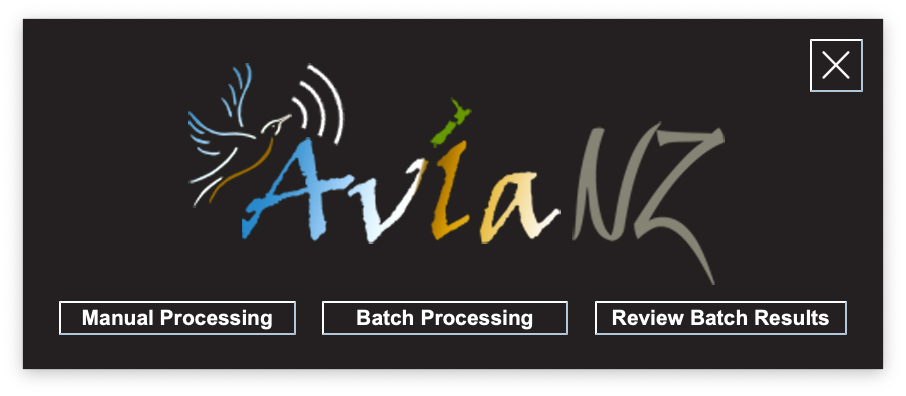
\includegraphics[width=.6\textwidth]{Figures/Splashscreen}
\end{center}

\begin{itemize}
\item The first option (`Manual Processing') is described more in Section~\ref{sec:manual}. It enables you to look at, listen to, and manually annotate individual audio files, as well as to train your own recognisers. 
\item The second option (`Batch Processing') takes whole directories (and subdirectories) of audio files and automatically segments the calls of selected species you have recognisers for; see Section~\ref{sec:auto}. 
\item You can view the output of the automatic segmentation using the the third option (`Review Batch Results', see Section~\ref{sec:review}), but if you want more context on them you could also use the first (`Manual Processing') option. 
\item The software can also produce an Excel file showing the results; these are described in more detail in Section~\ref{sec:outputs}. 
\end{itemize}

\newpage
\section{Manual Processing}
\label{sec:manual}

If you select `Manual Processing', you will see a dialog box asking you to select a file to view. Use this in the normal way to select a sound file from a directory. The program will then ask you to give names for the operator and reviewer. These are useful to keep track of who has looked at different files. Following that, you should see a screen like the one below. This is the main interface for manually labelling birdcalls, training recognisers, or testing things. It can also be used for reviewing the results of automatic processing; checking for misclassifications is usually easier in `Review Batch Results', but the manual processing mode also allows you to see if there are any calls that the recogniser missed and to correct the type of call and the time and frequency limits of the call.

AviaNZ can load sound files in wav format, or bat files in bmp format. Other sound files should be converted to wav format. Note that mp3 files lose a lot of information and should be avoided for bioacoustics recordings if possible, although they are what websites such as \url{http:www.xeno-canto.org} use. AviaNZ assumes that sound files are recording in mono (single microphone) sound. If there are other channels, it only loads the first one.

Very long recordings can be used, but it is generally easier if they are split into shorter files. We provide a splitter in the Utilies (see Section~\ref{sec:utilities}) but there are plenty of other options on the internet if you prefer.

\begin{center}
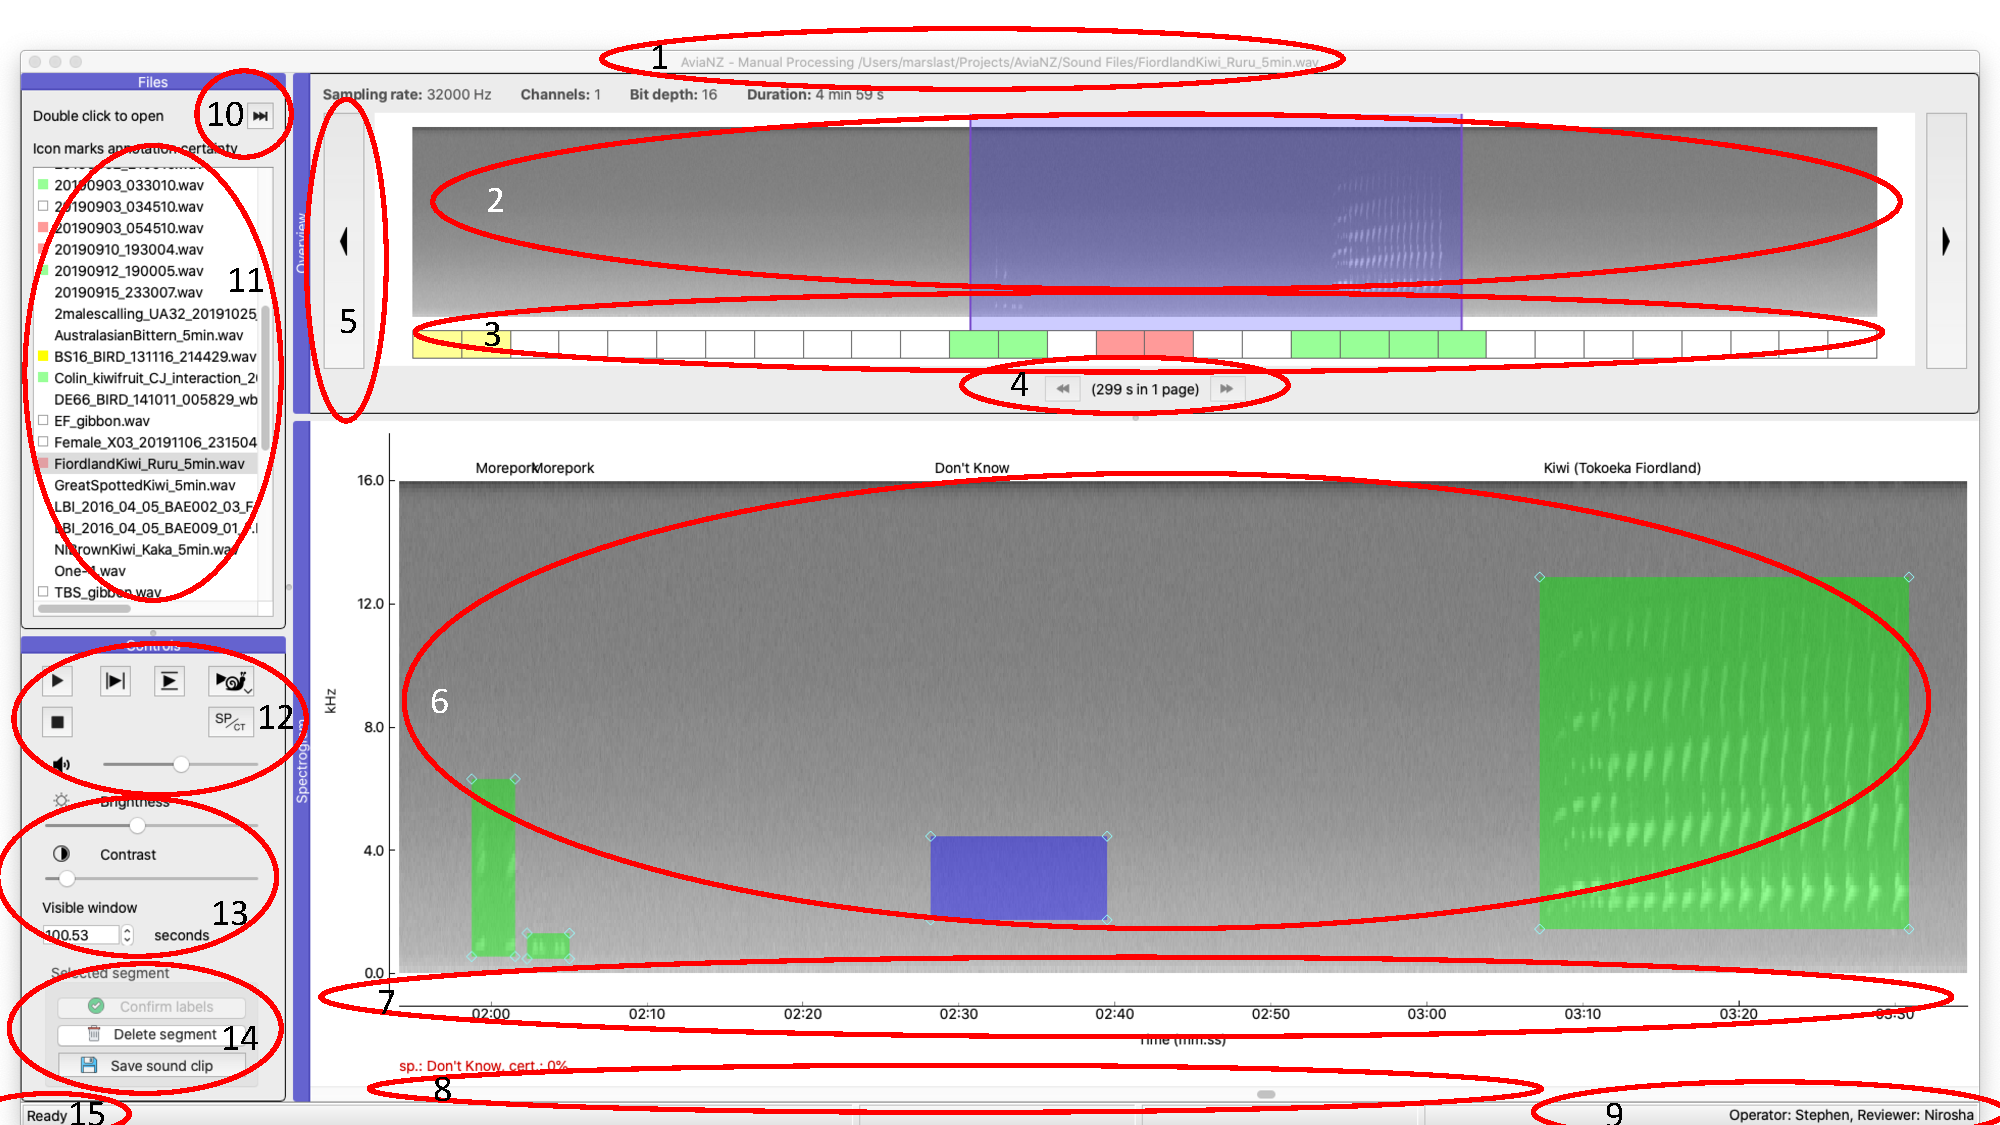
\includegraphics[width=.95\textwidth]{Figures/AviaNZInterface.pdf}
%\caption{The interface for manual processing and analysis.}
\end{center}

The name of the current file is shown in the title of the window (1). Below that there are four separate areas of the screen. Each has its name in a blue bar. They are:
	\begin{description}
	\item[Overview] This shows you a picture of a 5 minute segment of the file (labelled 2 in the figure). The part you are looking at in the main plots is shown in blue. The blue section can be moved by dragging the centre of the box, or resized by dragging the ends. Below the sound spectrogram there is a bar (labelled 3 in the figure). There are left and right arrow buttons on the sides of the image (labelled 5) and double arrow buttons (labelled 4) below. The single arrow buttons move the view in the main area along, while the double arrow buttons move to the previous or the next 5 minutes of the file (if they exist). 
	\item [Files (11)] This is a list of files in your current directory. You can double-click on one to select it and open it. We have added some more information about the status of the file in this version. Files that have not been opened in AviaNZ do not have an annotation to their left. Otherwise, a small box is shown. If the box is empty (white) then there are no segments of call annotated within it. If the box is green, then there are, and they all have species annotation. If the box is yellow then some are uncertain (either because the user added a question mark, or because an automated filter processed it and the output has not been confirmed). It the box is red then there are segments labelled as `Don't Know'. 

The double arrow button on the top right of this area (labelled 10) moves on to the next file.
	\item[Spectrogram (6)] This is the main representation of the sound file, and the way that you add and modify annotations. The axes for the image show frequencies on the vertical axis and time on the horizontal axis (7). The time is true time if AviaNZ can read that from the file, and starts from time 0:00 otherwise. It is possible to display information about where the mouse is pointing on the spectrogram (time, frequency, energy value) below the axis by choosing `Show pointer details in spectrogram' from the Appearance menu, and to switch it off the same way. There is also a scroll bar to move through the current page (8).
The way in which you annotate recordings is described in Section~\ref{sec:spectrogram}.
	\item[Controls] These play the sound file (12; see Section~\ref{sec:play}), modify the appearance of the plots (13 in the figure, see Section~\ref{sec:spectrogram2}) and process any segment that is currently selected by deleting it, confirming it's label, or saving it as a separate wav file (14).  For more details, see  Section~\ref{sec:play}.
	\end{description}

There is an optional fifth area, which is the Amplitude plot. If you want to see it, select `Show amplitude plot' in the Appearance menu. Select the option again to hide it. You can also hide the list of files (11) and the annotation overview (2--5) in the same way. AviaNZ will remember your choice in future uses.

There are two other parts to the interface:
	\begin{description}
	\item[Menu] The menu at the top of the screen. 
	\item[Status Bar] At the very bottom of the screen there is an area (15) that gives any status updates from the program, and on the right, information about the currently selected Reviewer and Operator (9).
	\end{description}

\begin{itemize}
\item You can drag the five screen areas around and reorder them if you wish, by dragging the blue bar on the top or left of them with the name of the section in it. You can also make them into their own windows by double-clicking on the blue bar. If you decide that you made a mistake doing that, then there is an option in the Actions menu to `Put docks back' that returns them to the original configuration.

\item To load a new file, either choose `Open sound file' in the File menu, or just double click one in the Files area (double clicking on a folder will open that folder; the `..' option at the top of the list takes you up one directory), or click on the button labelled 10 to move to the next file.

\item If you want to move to a new directory, either use the `..' option to navigate around your computer's file system, or use the  `Open sound file' in the File menu.

\item To restart the program, for example so that you can start doing some batch processing, choose `Restart Program' from the File menu. To quit completely, choose `Quit'. 
\end{itemize}

\subsection{Spectrogram}\label{sec:spectrogram}

\begin{itemize}
\item The main spectrogram plot (6) shows a section of a sound file. The part you are looking at is highlighted in blue in the top (Overview: 2) picture.

\item The axes of the spectrogram are time on the horizontal axis and frequencies on the vertical axis. The times will be true times if this information is available (such as when using DOC recorders), or time from start of file otherwise. 

\item Sometimes spectrograms don't look good initially, for example because of high noise. You can modify the brightness and contrast of the spectrogram using the two sliders in the Controls section (13). 
\item You can also use a different colour scheme, and invert the colour map (swap black and white), by choosing the relevant options in the Appearance menu.
\end{itemize}

\subsection{Zooming and Scrolling}

\begin{itemize}
\item The part of the file you can see can be changed by:
	\begin{itemize}
	\item dragging the scroll bar below the spectrogram (8).
	\item clicking on the left or right arrows on the right of the Overview picture (5).
	\item dragging the blue highlight in the Overview picture itself (2). 
	\item clicking on any of the boxes in the bar below the Overview picture (3).
	\item pressing the left or right arrow keys.
	\end{itemize}
	
\item The amount of the file that you can see (the visible width) can be changed by either: 
	\begin{itemize}
	\item dragging the ends of the blue highlight in (2).
	\item changing the `Visible window width (seconds)' in the Controls dock (14) by clicking on the up and down arrows, or typing in a new number.
	\end{itemize}

\item You can also view a restricted amount of the spectrogram by reducing the visible frequency band, see Section~\ref{sec:spectrogram2}. 
%To do this non-destructively, use the `Change spectrogram parameters' dialog in the Appearance menu, and change the Lowest and Highest Frequency options. There are other options in that dialog too, which are concerned with the way that the spectrogram is made.  For more information about them, see Section~\ref{sec:spectrogram}.
\end{itemize}

\subsection{Moving Through Long Files}

\begin{itemize}
\item If files are longer than 5 minutes, use the double arrows labelled (4) to move to the next or previous page, or press Shift + left or right arrow keys. 
\item The program tell you which page you are currently on, and many there are in total. 
\item There is a 10 second overlap between the pages. You can change the page size and the amount of page overlap by choosing the relevant options in the `Interface Settings' in the Interface menu, see Section~\ref{sec:interfacesettings}. 
\item The times on the axis below the spectrogram show locations in the full file.
\item Note that operations like denoising and segmentation (described in Section~\ref{sec:action}) apply to the visible 5 minute portion of the file, not the whole file.
\end{itemize}

\subsection{Manual Labelling (Sound Files)}

\begin{itemize}
\item To create segments, click and drag with the left mouse button on the Spectrogram. (The action of left and right mouse buttons can be swapped over in the Interface Settings.)
\item To select segments, click on them with the right mouse button (pressing control on the keyboard when clicking on a Mac). The segment will turn blue when it is selected.
\item If you find that the colours make it hard to see the data underneath the boxes you can make them transparent using the `Make dragged boxes transparent' option under `Annotation' in the `Interface settings'. You can also choose different colours if you have particular preferences.
\item Segments are saved automatically, so that you can't lose your work.
\end{itemize}

\subsubsection*{Creating and Labelling Segments}

\begin{itemize}
\item There are three ways to create a segment. You change which of them to use in the `Mouse settings' of the `Interface settings' in the Appearance menu:
	\begin{itemize}
	\item {\em (default)} Drag a limited frequency band box (i.e., click and hold the mouse button and drag the mouse to the correct end point in both time and frequency).
	\item Start and stop a limited frequency band by clicking (i.e., click once at the correct time and frequency for the start of a segment, and then again at the time and frequency for the end).
	\item Start and stop a full frequency band by clicking (i.e., click once at the correct time for the start of a segment, move the mouse to the end, click again, the box covers all frequencies).
	\end{itemize}
	
\item When you create a new segment, a drop-down menu will appear asking you to choose a label for that segment. 

\begin{itemize}
\item To choose the type of bird, click on the name. 
\item If the species isn't in the list, move to `Other'. 
\item If it isn't in the second list, at the bottom of that list is a selectable box (it probably says `Albatross'). Clicking on it provides the complete list of birds. 
\item If there is something missing from there, choose Other' from it, which is at the very end. It will ask you to enter a name, as Genus (Species); e.g., `Kiwi (Little Spotted)'. 
\item If there is only a single example of the genus, you can miss out the species, e.g., `Kakapo'. 
\item The new name you add will then appear in the list. 
\item If you click anywhere on the screen except on a bird name in the menu then the menu will disappear and the bird type will be labelled as `Don't Know'. 
\item The bird list that we are using is based on the one that DOC use, and is meant to cover all the bird species that we know about in New Zealand. 
\item You can add new species individually using `Other' in the menus.
\item It is possible to use other bird lists using the `Interface settings'.  
\end{itemize}

\item By default the lists of bird names update dynamically, so that bird types you have chosen appear at the top of the list. If you don't like that, then you can disable it in the `Interface settings'. 

\item When creating a segment, you can give it the same label as the previous segment by pressing the Shift key on the keyboard when you create the segment. The program will then give the segment the same label as the previous box that you labelled, without showing you the list. This is very useful when there is one bird calling repeatedly.

\item You can also show that you are uncertain by pressing the Ctrl button when you click to segment (command button on a Mac computer). The names of the birds will then have a question mark after them.

\item You can choose whether or not to allow more than one species per segment. This can be useful for recordings of the dawn chorus and where you just want to label presence of a set of species. Use the `Default to multiple species' in the `Interface settings' to allow this. Then, when you choose a bird from the list it will be ticked, and the menu will not close automatically, allowing you to make multiple selections. To unselect something, click on it again. When you make a new segment, `Don't Know' is selected by default. Choosing any other option deselects `Don't Know'. You can reselect it if you do want that label as well. 

\item {\em New to v3.0} AviaNZ now also allows you to specify the call type, which is something that is can be decided by the automatic analysis tools. This could be the difference between male and female vocalisations for e.g., kiwi, or different calls types such as `more-pork' or `cree' for ruru. The choice of which call types are available is made in the automatic filter, which is covered in Section~\ref{sec:trainfilter}. To swap between seeing the species and seeing the call use the SP/CT button (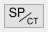
\includegraphics[scale=0.5]{Figures/SPCT}) on the right of area 12 of the Controls panel.
\end{itemize}

\subsubsection*{Updating Segments}

\begin{itemize}
\item If you select a segment that already exists by clicking on it then it will turn blue. Click on it again and the menu will reappear so that you can correct mistakes. This will be either the species label or the call type label depending on the SP/CT button.
\item Segments have blue diamonds at the corners, so that you can resize them, or you can move the whole segment by dragging it (this works even when it isn't selected). 
\item Segments can be deleted by selecting them (so that they turn blue) and then clicking on the `Delete Current Segment' in the Controls or pressing the delete or backspace key on the keyboard. 
\item To delete all of the segments from the current file, use the `Delete all segments' option in the Actions menu. 
\item You can disable the making and updating of segments (to avoid making segments by mistake) by selecting `Make read only' from the `Appearance' menu.
\end{itemize}

%You can denoise a single segment by selecting it, and then pressing the button with a paint brush on in the `Controls' section (14).

%\item The button with a small `i' on in the `Controls' section (14) changes the information that is shown about each segment; rather than the species label, the syllable name from the recogniser is given. The drop-down list then changes to enable you to correct this instead if there are any options to do so. 

\subsubsection*{Colour Codes}

\begin{itemize}

\item The segments that are drawn on the screen have different colours. These colours are changeable in the `Interface settings', but by default are:
	\begin{description} 
	\item[Blue] This segment is currently selected. You can play it by pressing the buttons in the Controls area (see Section~\ref{sec:play}), or give it a new label by clicking on it again, or delete it. 
	\item[Green] This segment has been labelled with a bird name, either manually, or by an automatic filter that has high confidence in the result.
	\item[Yellow] This segment has been labelled with a bird name with a question mark, or an automatic filter is unsure but thinks it is possible. 
	\item[Red] This segment has been labelled as `Don't Know'.
	\end{description}

\item These colours match the rectangles underneath the Overview:

\begin{center}
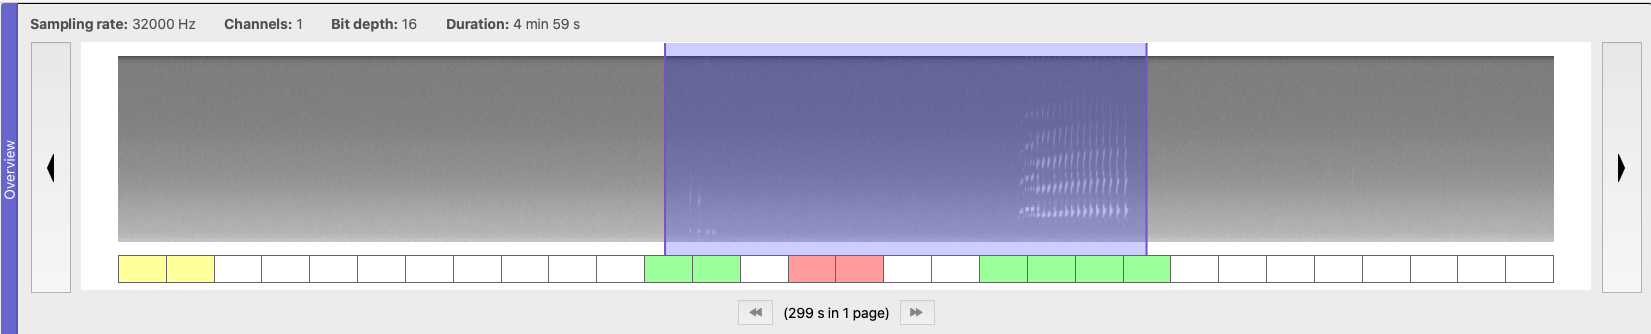
\includegraphics[width=.9\textwidth]{Figures/Overview}
\end{center}

\item For each 10 second segment of the file, these boxes are:
	\begin{description} 
 	\item[White] if there are no segments, or
	\item[Red] if there are `Don't know' segments, or
	\item[Yellow] if there are question-marked segments, or 
	\item[Green] if all the segments in that section are labelled with definite species. 
	\end{description}
	
\item You can click on those boxes, and they will update the main spectrogram plot to show that section of the file. This is a useful way to move through the file quickly.
\end{itemize}

\subsection{Manual Labelling (Bat Files) \label{sec:bats}}

\begin{itemize}
\item In v3.0 AviaNZ can also process bat files saved by DOC AR4 recorders (in .bmp format). 
\item When a bat file is loaded, the full length of the file will be shown, and the frequency range expanded up to 88 kHz. Guidelines will also be drawn on the screen to match the ones shown in DOC's BatSearch program. 
\item AviaNZ automatically makes a single segment that covers the detection for you. You can't see the segment, but you can see the `Don't Know' label at the top of the spectrogram. Click anywhere on the spectrogram, and a menu will drop down so that you can label the species. If you view it as a `possible' option then press the control key when you click to add a question mark to the label.
\item You can delete the segment, but you can't add new ones or resize this one, the annotation is given to the whole recording.
\item If you want to listen to a Bat call, there is an option to `Save sound file' in the Actions menu. This will create a sound file with the same name as the original file, but with a .wav extension. This can then be played as a sound file. We have slowed the recording down so that you can hear the bat sound in human audible range. Note that the quality of the sound file is not particularly high because of the way that the files are stored by the AR4. 
\end{itemize}

\subsection{Controls \label{sec:play}}

\begin{center}
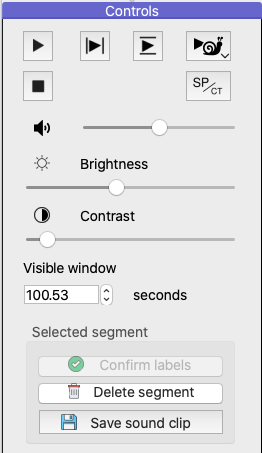
\includegraphics[width=.25\textwidth]{Figures/Controls.png}
\end{center}

\begin{itemize}
\item The buttons at the top of the controls block allow you to play the sounds. 

\begin{itemize}
\item The top-left button is a normal play button. The button turns into a `Pause' button while playing.  
\item While the sound is playing, the light blue bar in the spectrogram plot shows where the playback is up to. 
\item When the sound is paused, you can drag this bar if you want to hear a particular part of the file. Move the mouse over it, and the bar will go red. Then click and drag (using the mouse button that does not make segments, by default the right button) to move it. 
\item To stop playback and have the slider return to the start of the visible section, press the Stop button.
\item When a segment is selected (so that it is blue) you can use the three play buttons to the right of the stop button to play just that small segment. 
\item The difference between these is:
    \begin{itemize} 
    \item the one on the left (
\includegraphics[scale=0.3]{Figures/playsegment}) plays all the frequencies in the sound file
    \item the one in the middle (
\includegraphics[scale=0.3]{Figures/playBandLimited}) plays only the frequencies highlighted, so that you can isolate particular frequencies of a call. This is particularly helpful when there is high level of background noise in a particular frequency range, such as cicadas, or where there are overlapping calls in different frequency bands.
    \item the one on the right (with the snail: 
\includegraphics[scale=0.03]{Figures/playSlow-w}) lets you play the segment at different speeds. Hold the button down to change it to 2x (twice as fast) or 1/2 or 1/4 speed. Note that the pitch also changes, but it can be interesting or useful to hear all the components of a call.
    \end{itemize}
\item You can change the volume of playback using the slider below the buttons. 
\item The SP/CT button changes whether you control species labels or call type labels of the segments.
%\item The button that shows a brush denoises a segment to try and make it easier to hear the bird call.
\end{itemize}

\item The brightness and contrast sliders change the appearance of the spectrogram, helping to see more sounds. 
\item The size of the visible window controls how much of the full spectrogram appears in the main window.
\item The `Confirm labels' button makes a segment label certain. This is useful to confirm labels that were made by an automatic recogniser, or that the user was previously unsure about.
\item The `Delete segment' button removes any segment that is selected (blue colour). 
\item The `Save sound clip' button saves a selected segment as a short sound file.
\end{itemize}

\subsection{Menu Options}	

Most of the options for AviaNZ are found through the menus. There are keyboard shortcuts for many of the menu items, which can be seen in the menus themselves. 

\subsubsection{{\em File Menu}}

\begin{center}
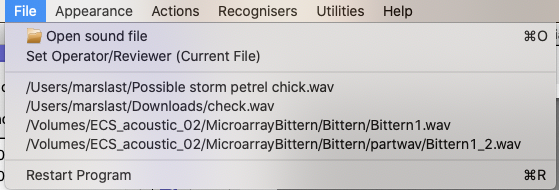
\includegraphics[width=.7\textwidth]{Figures/FileMenu}
\end{center}

\begin{description}
\item[Open sound file] Produces a file dialog so that you can choose a new sound file to open.
\item[Set operator/reviewer (Current File)] Enables you to change the operator or reviewer that were specified when you started AviaNZ. The change only applies to this file. 
\item[List of recently used files] Makes it easy to revisit recent files.
\item[Restart program] Takes you back to the start screen so that you can access the other functions.
\item[Quit] Does what it says.
\end{description}

\subsubsection{{\em Appearance Menu}}

\begin{center}
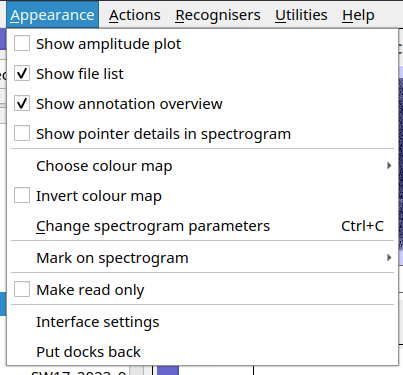
\includegraphics[width=.5\textwidth]{Figures/AppearanceMenu}
\end{center}

\begin{description}
\item [Changing appearance] The first four options in the menu hide or reveal the amplitude plot, list of files, overview, and information about where the mouse is pointing in the spectrogram. The ones that are selected are marked with a tick. 
\item [Choose colour map] This enables the user to select a colour map they prefer to the standard grey one. 
\item [Invert colour map] By default, areas of high energy (frequencies where there is a call or other sound) are shown as the lightest colour, and low energy as dark. This can be swapped over with this option. Note that you will need to change the brightness and contrast using the controls area after inverting the colour map.
%\item [Make frequency axis tight] After bandpass filtering, this updates the spectrogram plot to stop showing the empty bands.
\item [Change spectrogram parameters] A set of options to modify the spectrogram.  See Section~\ref{sec:spectrogram2} for more details. %Enables changes of the windowing function, width and increment of the FFT, and the option to not subtract off the mean. The `Multitapering' option can make very noisy spectrograms look better, but it takes a lot of computer time. 
The two sliders at the bottom of the dialog enable the user to non-destructively show a limited frequency band in the spectrogram. The axis in the plot shows the range that is visible. 
\item [Mark on spectrogram] There are some features that will help you spot bird calls or recognise them. We currently offer three options here: the fundamental frequency, spectral derivatives, and points of high energy. To select one, choose it from the menu; select it again to remove it. They can help to find particular types of call. 
\item [Make read only] When reviewing a segmentation it is possible to click on the plots by mistake, adding further segments. This option avoids this problem. It can be turned off by selecting it again. When read only mode is on, the message section at the bottom of the screen says so. 
\item [Interface settings] This option produces a dialog that enables the user to customise several things about AviaNZ. See Section~\ref{sec:interfacesettings} for more details.
\item [Put docks back] Returns the various screen components to their original layout if they have been moved around. 
\end{description}

\subsubsection{{\em Actions Menu}}
\label{sec:action}

\begin{center}
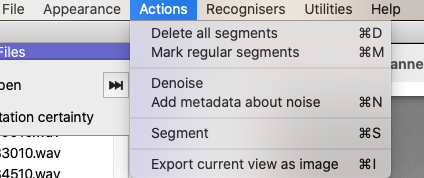
\includegraphics[width=.5\textwidth]{Figures/ActionsMenu}
\end{center}

These options will mostly provide dialog boxes that ask you to make choices. 

\begin{description}
\item [Delete all segments] Does what it says. 
\item [Mark regular segments] Some users find it helpful to have an automatically generated segment box at regular intervals, for example to label all the birds in that segment under some statistical protocol. By default these are boxes are made to be 15 seconds long, with one box every 300 seconds (5 minutes) through the file. These options can be changed using the `Check-Ignore protocol' area in the `Interface settings'. There is also an option there to simply mark those areas rather than putting a segment box in place.
\item [Denoise] Runs some programs that try to get rid of the noise in the sound file so that the birdcalls are easier to see. %You can also denoise a single segment by selecting it, and then pressing the button with a paint brush on in the `Controls' section (14). 
See Section~\ref{sec:denoising} for more information.
\item [Add metadata about noise] Allows the user to specify if the sound file is particularly corrupted by noise, and also to identify the type(s) if known. This can be an optional data field, or made compulsory for each file by choosing the appropriate option in the `Interface settings'.
\item [Segment] You can ask the computer to segment the calls automatically. We currently provide 3 options. The first (`Wavelets') applies a pre-trained recogniser for a particular species, in the same way that the Batch Processing mode (Section~\ref{sec:auto}) does, but just to the current page. The other two (`FIR' and `Median Clipping') will create a segment for any significant noise in the file. 
%\item [Export segments to Excel] This enables the user to save a summary of the annotation of the currently opened file into an Excel workbook (in the same location as the current sound file), as is described in Section~\ref{sec:outputs}. 
%\item [Find Matches] If you select a segment (so that its box is green) and then press this button the program will look for others that are similar. It does not currently deal well with nosie. 
%\item [Filter Spectrogram] This tries to clean the spectrogram for easier viewing.
%\item [Calculate segment statistics]
%\item [Human Review] These two options provide two different ways to view the segments and their labels on the current page for easier checking. For more, see Section~\ref{sec:review}.
%\begin{description}
%\item[All segments] Show each segments regardless of label.
%\item[Choose species] Show all segments for one species.
%\end{description}
\item [Export current view as image] Saves the spectrogram currently visible on the screen as an image, including any segments marked. 
\end{description}

\subsubsection{{\em Recognisers Menu}}

\begin{center}
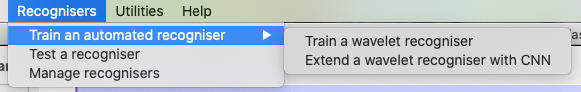
\includegraphics[width=.7\textwidth]{Figures/RecognisersMenu}
\end{center}

\begin{description}
\item [Train an automated recogniser] A significant new feature of this version of AviaNZ is that you can now train your own species recognisers. The process is as simple as we can make it. It is described in Section~\ref{sec:trainfilter}. Please read that section before using this feature.
\item [Test a recogniser] Enables you to test a recogniser by choosing a folder to run it on. See Section~\ref{sec:testfilter}.
\item[Manage recognisers] Lets you rename, export, or import new recognisers for different species. 
If you have made recognisers for sounds that you think will be useful for other people, please upload them to our AviaNZ webpage.   
\end{description}

\subsubsection{{\em Utilities Menu} \label{sec:utilities}}

\begin{center}
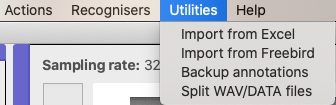
\includegraphics[width=.4\textwidth]{Figures/UtilitiesMenu}
\end{center}

\begin{description}
\item [Import from Excel] If you have made user annotations in other programs that you want to import, this option will help to do it. Normally you can export annotations in csv or excel format, and then load them into AviaNZ using this option.
\item [Import from Freebird] For the Freebird software, you can import user annotations directly.
\item[Backup annotations] If you want to copy a set of user annotations (for example to have them backed up, or to transfer them to another computer) without the wav files, but with the directory structure preserved, this option will do that. 
\item[Split WAV/DATA files] DOC AR4 recorders produce 15 minute sound files, but many other recorders produce far longer recordings. This can mean that you spend a lot of time going forward and backward through spectrogram pages. This option lets you split the sound files into shorter pieces. If you have already processed them, so that they have segments included, there will also be transferred to the new sound files.
\end{description}

\subsubsection{{\em Help Menu}}

\begin{description}
\item [Help] Gives access to this manual online.
\item [Cheat sheet] Links to our webpage to see examples of New Zealand bird spectrograms and calls.
\item[About] Shows you basic information about AviaNZ.
\end{description}

\subsection{Changing the Spectrogram Computation}\label{sec:spectrogram2}

\begin{itemize}
\item Selecting `Change spectrogram parameters' from the Appearance menu will produce the following dialog box:

\begin{center}
    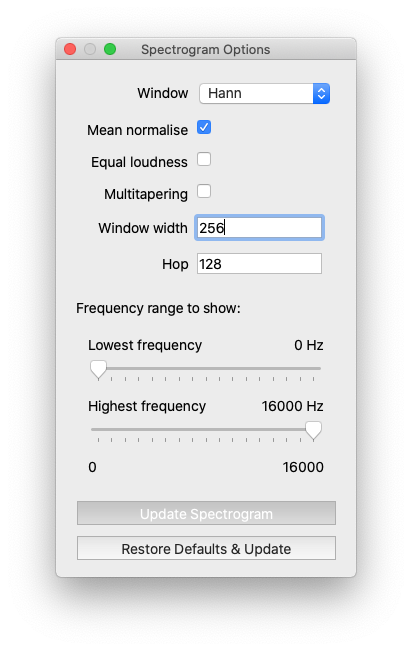
\includegraphics[width=.5\textwidth]{Figures/SpectrogramOptions}
\end{center}

\item You can change some of the parameters that are used to produce the spectrogram:

\begin{itemize}
\item The window function (default: Hann) controls how the spectrogram combines sounds across the time range. 
\item Mean normalisation and equal loudness try to make the spectrogram energies more even.
\item Multitapering uses multiple windows to make a better estimate of the spectrogram, but performs a lot of computation, and can therefore be slow.
%\item Spectrogram reassignment also tries to make a better estimate.
\item The window width and hop size control how much of the sound file makes up one spectrogram bin, and how they overlap. A big window size will improve frequency resolution, but reduce time resolution, and vice versa. The hop size controls how much the spectrogram time bins overlap. It is computationally more efficient if these numbers are powers of 2 (such as 256, 512, 1024).
\item The frequency range sliders let you change the visible frequency range in the main spectrogram window. This can be useful if you want to focus on only part of the range.
\end{itemize}

\item If you want to know more about these options, look on the AviaNZ webpage, in the `Technical Details' section. 
\item You can also just try changing them and see if it makes your spectrograms clearer.
\end{itemize}

\subsection{Denoising}\label{sec:denoising}

\begin{itemize}
\item When sound files are particularly noisy, it can be helpful to remove some of that noise. AviaNZ currently provides three ways to do this (via the `Denoise' option in the Actions menu):
\begin{description}
\item[Wavelets] This is our main method, and tries to preserve the bird call perfectly. 
\item[Bandpass] Suppresses all frequencies outside a restricted range (which you specify) so that you can concentrate on the frequency range where calls that you are interested in can be seen.
\item[Butterworth bandpass] Another way to compute a restricted frequency range.
\end{description}
\item You can save the denoised sound files, and undo the denoising if it does not help.
\end{itemize}

\subsection{Interface Settings}\label{sec:interfacesettings}

\begin{itemize}
\item There are quite a few user-selectable options in AviaNZ, which you can choose using the `interface settings' menu option in the Appearance menu, which will produce the following dialog box:
\begin{center}
    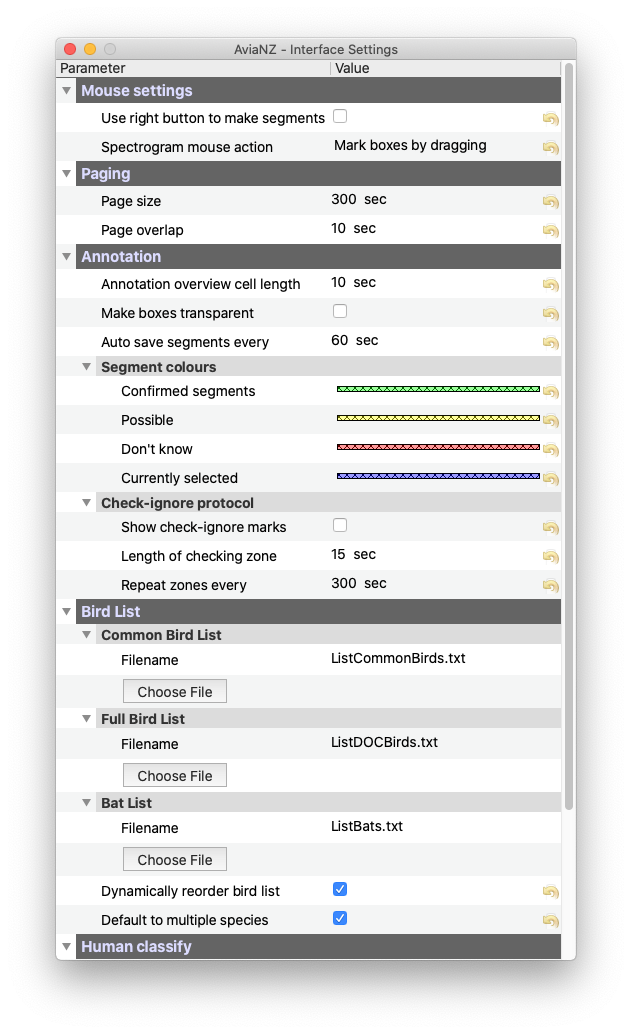
\includegraphics[width=.65\textwidth]{Figures/InterfaceSettings}
\end{center}

\item These options include:
\begin{description}
\item[Mouse settings] Swap which mouse button selects segments and which creates them, and change the method of creating segments (clicking or dragging).
\item[Paging] The page is the length of spectrogram loaded into AviaNZ at one time. By default it is 300 seconds (5 minutes). Note that longer times will require more memory and processing time. The amount of overlap between the pages can also be specified. The aim of the overlap is to make sure that calls aren't missed, and that segments are labelled accurately, at the page limits. 
\item[Annotation] 
\begin{itemize}
\item The first option in this section changes the length of the boxes in the Overview. 
\item The next enables you to make the labelling boxes transparent (so that only the outline of the box is shown) if you find it hard to see what is in a segment. 
\item By default, AviaNZ save the segments you have made every 60 seconds. This can be changed, for example if you want to do it more often for safety. 
\item You can also change the colours of segments.
\item AviaNZ has a check-ignore protocol for people who only annotate subsets of recordings. This puts a mark on the spectrogram in places where the user should be annotating the spectrogram, which you can control with these options.
\end{itemize}
\item[Bird list] There are two bird lists in AviaNZ: the short list of common birds, and a longer list of all possibilities, together with a bat list. You can change these files for others (for example, to include non-New Zealand species). %See Section~\ref{sec:birdlists} for more information. 

You can also change the default behaviours of dynamically updating the list of common birds, and enable multiple species to be selected for a single segment. This can be useful for labelling things like the dawn chorus, but these segments will not provide good training data for new recognisers. 
\item[Human classify] By default, AviaNZ saves corrections that are made using the review options (see Section~\ref{sec:review}). 
\item[User] Enables you to set the operator and reviewer; this facility can also be found in the File menu. You can also change whether or not the AviaNZ window starts at full screen size, and whether or not the noise data must be completed for all files. 
\end{description}
\end{itemize}

There are two other ways to interact with AviaNZ. They are selectable via the start screen, and are described next.

\newpage
\section{Batch Processing}
\label{sec:auto}

Batch processing is for use when you have large numbers of recordings that need to be processed, for example when you collect recorders from the field. After downloading all of the data from the SD cards into a folder on your computer, start AviaNZ. 

\begin{center}
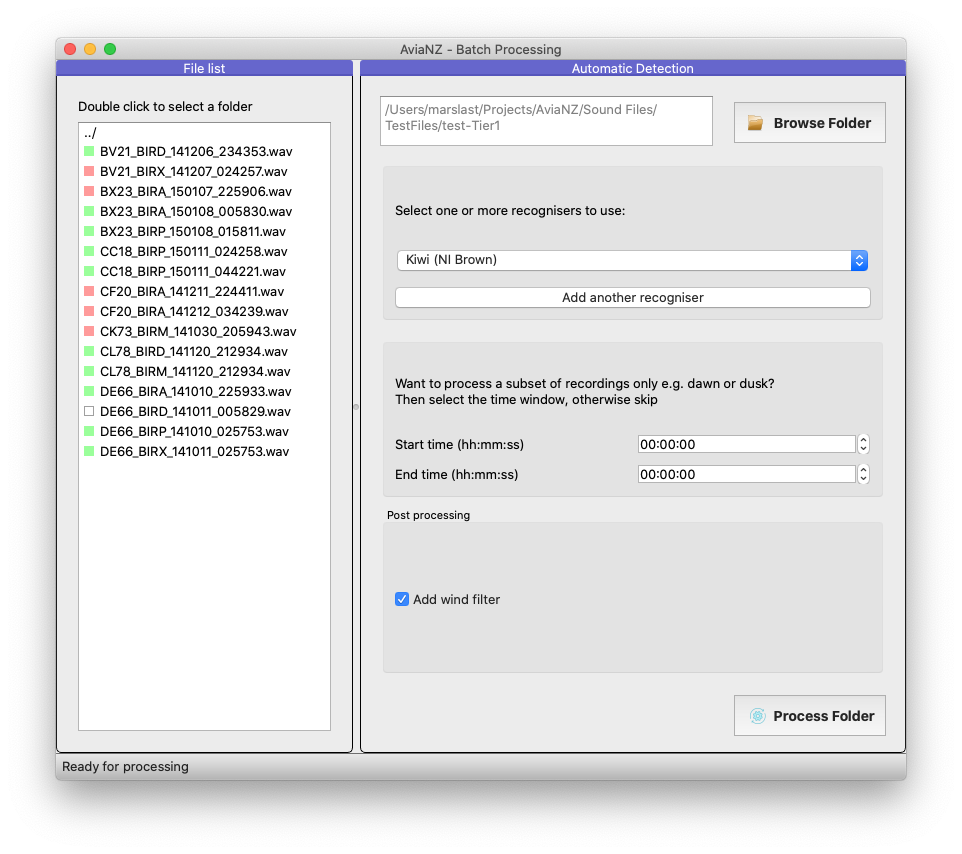
\includegraphics[width=.95\textwidth]{Figures/BatchProcessing}
\end{center}

\begin{itemize}
\item Select `Batch Processing' from the starting window. You will see a screen like the one above. 
\item Navigate to a folder containing recordings to process. 
\item If this folder contains subfolders, the program will work through all of the folders inside the original one. 
\item Note that it deletes any previous annotations in your files. If you want to save them, use the manual mode and the `Utilities $\rightarrow$ Backup annotations' option.
\item There are two outputs from batch processing: the data files that AviaNZ uses to label segments, and Excel files annotating the presence or absence of different species (see Section~\ref{sec:outputs}).
\item You can choose one or more species-specific recognisers from the drop-down list to apply to the sound files in order to automatically label them. 
\item Alternatively, you can select `Any sounds'; in this case AviaNZ will show any sounds in the files, and label them as `Don't Know'. 
\item For recordings from DOC recorders you can also choose to limit the times of the recordings. 
\item You can choose whether or not to try and filter out the sound of wind. This is useful if your data was collected in a windy place, but may miss some calls otherwise. 
\item Note that the `Any sounds' option will delete the Excel files for individual species to ensure that everything is consistent. The information is then held in one spreadsheet.  
\item The `Any sounds (Intermittent sampling)' option shows regular segments based on the `Check-ignore protocol' settings in the `Interface setting' in Manual mode, which is 15 seconds every 5 minutes by default. This provides another way to perform some manual annotation quickly and easily.
\item Press the `Process Folder' button to start the program. This is a very computationally intensive process, and will take a long time (hours) if there are lots of files to process, and make your computer hard to use for anything else. If you have a lot of files it do this kind of processing overnight. 
\item If you stop the processing partway through, AviaNZ will try and restart from the place it got up to last time if you restart it.
\item Once it has finished, the window will give you the option to see the AviaNZ start screen again so that you can review the outputs. You can either do this in the `Manual Processing' interface, or use the `Review Batch Results' option, which is described next. 
\end{itemize}

\section{Review Batch Results}\label{sec:review}

After batch processing it is important to verify the results, since AviaNZ will have created false positives (labelled calls are being your species when they are not). We try not to have too many false negatives (missed calls) because they are harder to find later. However, this does mean that there are more false positives instead. We provide two interfaces for checking and correcting the results. 

If you select `Review Batch Results' on the start screen then the following window will appear.

\begin{center}
	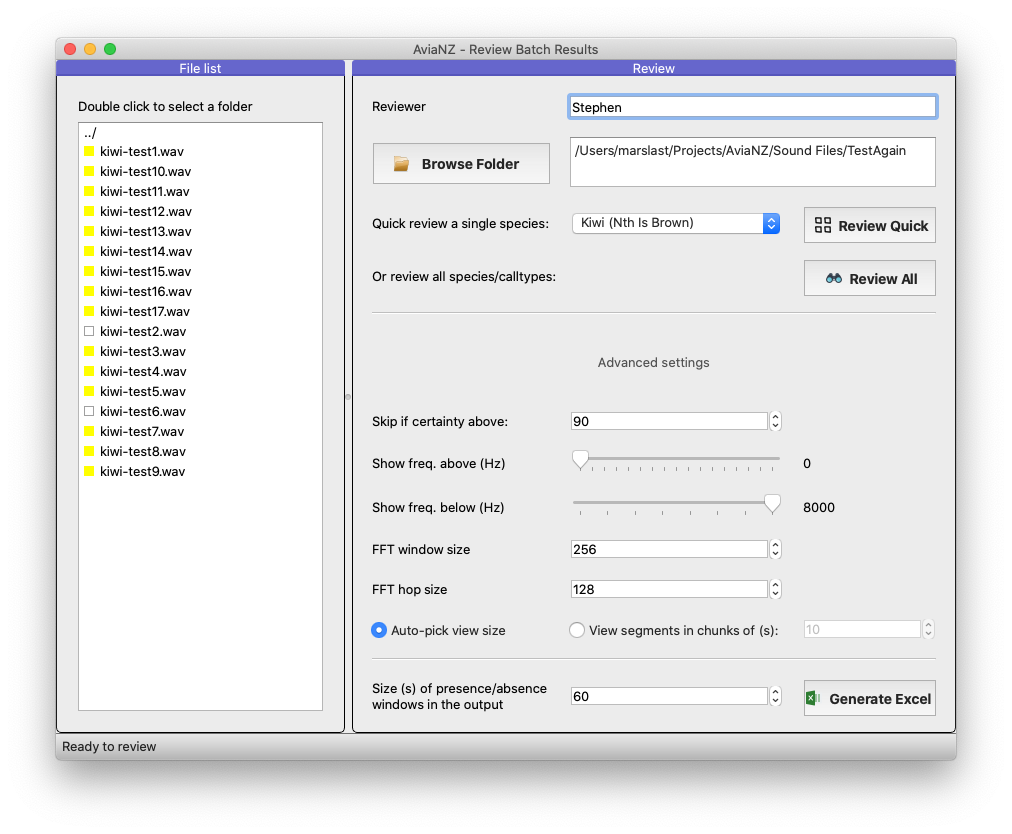
\includegraphics[width=.95\textwidth]{Figures/BatchReview1}
\end{center}

\begin{itemize}
\item Give a reviewer as in the Manual interface, then browse to a folder of previously processed files that you wish to review.
\item `Quick review' is designed to let you process lots of files quickly to remove false positives. It shows only the spectrograms related to the species selected in the drop-down box, see Section~\ref{sec:batchQuick}.
\item `Review all' is designed to let you see more detail about each segment, including potentially the call type as well as species. See Section~\ref{sec:batchAll}.
\item The option marked `Skip if certainty above' is important. AviaNZ assigns a confidence score to its classification of a bird call. User annotations, and automated annotions that the user has confirmed, are scored 100. Classifications by just a wavelet-based recogniser are scored 50, as are annotations with a ? on by the user. Neural-network based automated annotations have confidence assigned by the neural network. If you want to see all annotations you should set this parameter to 100 (the maximum value). If you wish to only see those that the system is not certain of, the default of 90 is suitable. As you set the value lower, more and more of the detections will be suppressed. Below 50 there will not be any segments to review.
\item At the bottom of the window is the option to generate an Excel file of outputs; see Section~\ref{sec:outputs}.
\item There are also a variety of options to change the appearance of the spectrogram in the Advanced Settings. These act in the same way as was described in the Manual interface section.
\end{itemize}

\subsection{Quick Review\label{sec:batchQuick}}

\begin{center}
	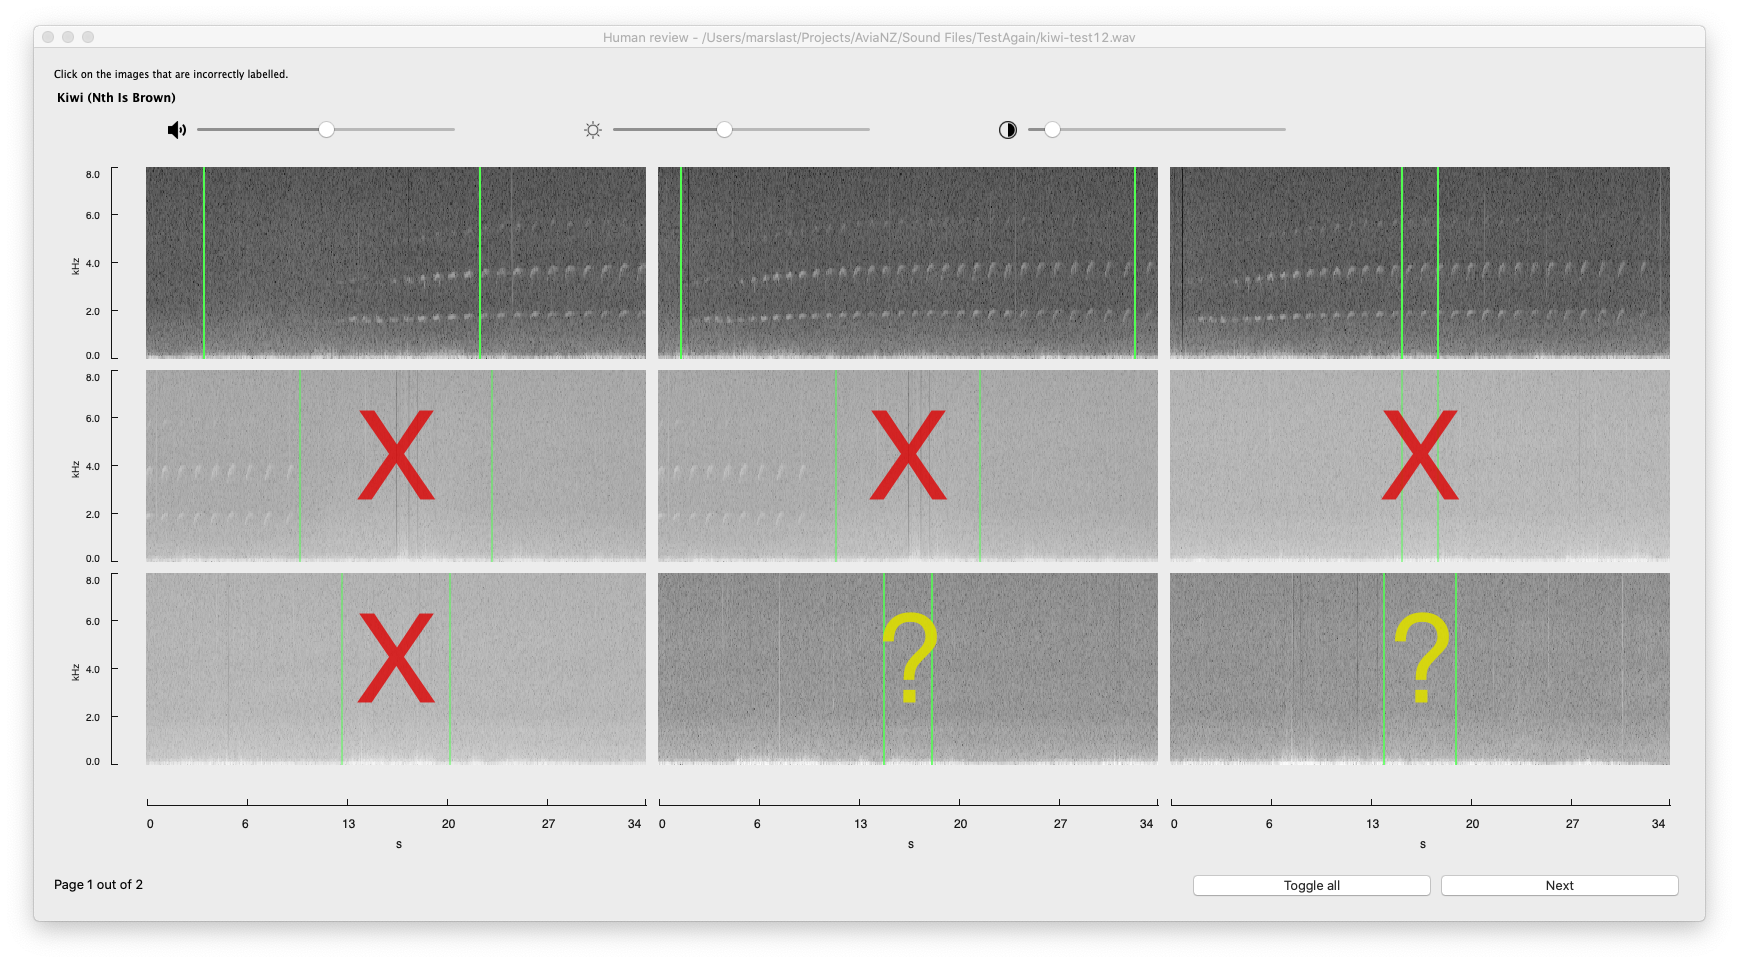
\includegraphics[width=.9\textwidth]{Figures/BatchReview2}
\end{center}

\begin{itemize}
\item The quick review mode is intended to let you delete false positives quickly. 
\item A set of spectrograms that have been labelled as your chosen species are shown. You can specify the size of these in the Batch Review interface above (by selecting `View segments in chunks of (s)') or let AviaNZ choose it (`Auto-pick view size').
\item Make the window larger to see more of them, any that do not fit will be shown on another page. 
\item For each segment that is wrongly labelled, click on its picture (it will be marked with a cross). 
\item If you click on it again, the cross will become a question mark to show that you are unsure, and if you click again, it will return to having no mark. 
\item Segments marked with a cross will be deleted, those with a question mark will be identified as unsure by having a question mark added to those label (confidence 50), while those left plain will be confirmed as correct. Using the question mark option is useful to then review them further in either the All Species review (Section~\ref{sec:batchAll}) or the Manual interface.
\item You can change the brightness and contrast at the top of the screen.
\item You can also play the sounds by hovering on the image, and then clicking on the play button at the top-left of the image when it appears. 
\item The `Toggle all' button cycles all of the spectrograms through the cross-question mark-OK stage, so that you don't have to click on every button if there are a lot of errors. 
\item Click on `Next' to move on to the next screen, which will either be more spectrograms from this file, or move on to the next file. 
\end{itemize}

\subsection{Review All Species\label{sec:batchAll}}
\begin{center}
	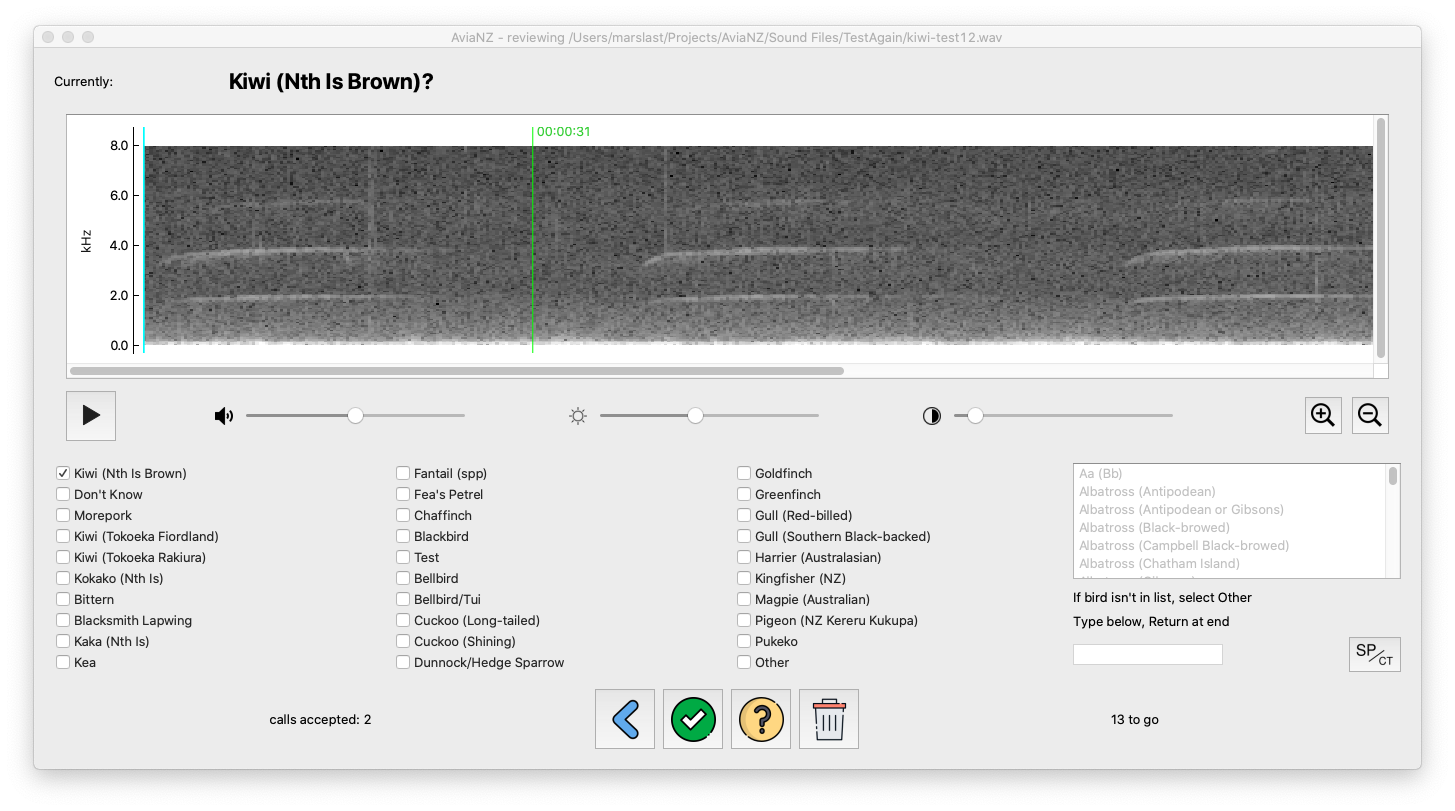
\includegraphics[width=.95\textwidth]{Figures/BatchReview3}
\end{center}

\begin{itemize}
\item The all species review is intended for a more in-depth review. You can also change the call type as well as the species using the 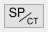
\includegraphics[scale=0.5]{Figures/SPCT} button.
\item The green bars on the spectrogram show the start and end of the call; the spectrogram includes a couple of seconds of context sound too. 
\item If the spectrogram is too large then the window will scroll. You can use the `+' and `-' buttons (with a magnifying glass on) to zoom. 
\item You can play the sound with the play button. 
\item You can also change the spectrogram brightness and contrast to make it easier to review. 
\item If the label is correct, click on the green tick, which will make the next image load. 
\item If the label is wrong, select the correct label before clicking the tick button. 
\item If you are unsure, or want to mark the segment for further attention (for example, because it includes other sounds and you want to resize it) then press the question mark button (
\includegraphics[scale=0.03]{Figures/questionL}). It is then easy to find in the Manual interface later.
\item If you have allowed multiple species selection (in the `Interface setting' in the Manual Interface) you can pick several options. 
\item To delete a segment, click on the red dustbin button. 
\item To move back to the previous one, click the back arrow; note that this will not save your current changes. 
\end{itemize}

%\item You can also see these two types of review from the `Manual Processing' interface by selecting `Human review' and then either `All segments' or `Choose species'. 

\subsection{Outputs}
\label{sec:outputs}

The AviaNZ program aims to provide detailed and easy-to-review outputs. An Excel file (with the name `DetectionSummary' followed by the species selected) will be generated with three sheets of outputs in the same directory as the files. If this file already exists, the new results will be appended to the end of each sheet. 

The three sheets of the Excel workbook are:
\begin{enumerate}
\item start and end times of each birdcall detected
\item presence/absence of the target species (or set of species) in each recording
\item  presence/absence of the target species (or set of species) in each time interval that the user specifies (by default 60 seconds)
\end{enumerate}

In addition to the Excel file, for each sound file AviaNZ generates an annotation file of the automated detections that  the user can open and review in either the main interface or using the `Review Batch Results' option. 

\newpage
\section{Training a species recogniser}\label{sec:trainfilter}

\subsection{Overview}

One of the main features of AviaNZ is that you can train your own species recognisers for use in batch processing. You can also swap them between people.% At the moment these recognisers are fairly simple; they are intended to include {\em any} sound that might be a call from the species of interest. However, over time we will be working to improve them so that they are more accurate, while still being easy to train. 

The process of training filters is fairly complex, and can be computationally expensive. The quality of the final filter depends on the training data used, the quality of the labelling that was performed, how noisy the files are, and how many other birds there are present.

AviaNZ has two levels of filters. The first is the wavelet filter. This does not need too much data to train, but will usually produce a lot of false positives. You can stop at this stage, but it you want to get higher accuracy, then you can train a second level filter, which refines the first by using a neural network. This requires a lot of data and training time. In both cases there are three parts to training a filter:

\begin{enumerate}
\item Creating training labels
\item Running the training process
\item Testing the recogniser
\end{enumerate}

Once these have been completed, the filter will be saved, and can then be used in the recognition process using `Batch Processing'. 

Before we start considering the process of training, it is useful to understand how to interpret the outputs that AviaNZ gives you. 

\subsection{Some important concepts}\label{sec:metrics}

The way that AviaNZ decides whether or not it has recognised a call correctly is by comparing it with human annotation. The training sound files that you provide, together with their annotations, are used to recognise the characteristics of the calls of a particular species. Comparing the human and machine outputs, there are four possible outcomes for each second of the recording:

\begin{center}
\begin{tabular}{lllll}
&          &  & \multicolumn{2}{c}{\textbf{Human}}   \\
\cmidrule(lr){4-5}
             &          &  & \multicolumn{1}{c}{Call}                                               & No Call                                                               \\
 \textbf{AviaNZ}                  &\vline \hspace{0.25cm}Call     &  & \textit{True Positive (TP)}  & \textit{False Positive (FP)} \\
                  &\vline \hspace{0.25cm}No Call &  & \textit{False Negative (FN)} & \textit{True Negative (TN)}  \\
\end{tabular}
\end{center}

\begin{description}
\item[True Positive (TP)] AviaNZ and human agree that there was a call 
\item[True Negative (TN)] AviaNZ and human agree that there was not a call
\item[False Positive (FP)] AviaNZ says that there was a call, but the human did not
\item[False Negative (FN)] AviaNZ did not detect a call that the human found
\end{description}

The counts of how many seconds of the recordings correspond to each of these four quantities can be combined to produce a variety of measures of accuracy, including:

\begin{description}
\item[Specificity (True Negative Rate)] $= \frac{TN}{(TN + FP)}$ (number correctly labelled as negative / actual number of negative examples)
\item[Recall (Sensitivity or True Positive Rate)] $= \frac{TP}{(TP + FN)}$ (number correctly labelled as positive / actual number of positive examples) 
\item[False Positive Rate] $= 1 - \mathrm{Specificity} = \frac{FP}{(TN + FP)}$ (number incorrectly labelled as positive / actual number of negative examples)
\item[Precision] $= \frac{TP}{(TP + FP)}$ (number correctly labelled as positive / number labelled as positive)
\end{description}

Not all of these metrics are truly useful for birdsong recognition, mostly because there are usually far more seconds in a field recording without any bird calls in that there are with the calls, and so the true negatives swamp the calculations. The two of most interest are recall, which counts the percentage of the calls that were found by the program, and precision, which counts the percentage of the calls found that were correct. Ideally both recall and precision would be close to 100\%, but there is a trade-off between them, so it is hard to do both at once. For the first part of the recognition process we aim to detect as many of the calls as possible (high recall), which can lead to lower precision. 

We also compare the True Positive Rate and False Positive Rates to assist in parameter setting, as we shall see shortly.

\subsection{Labelling}

In order to start the training process, you need to start by performing some manual labelling of calls of your target species in the Manual Interface.

\begin{description}
\item[Preparation] Select some sound files for training and testing. 
\begin{itemize}
\item The selection of sound files for training, and the careful labelling of the calls within those sound files, has the most potential for making a good recogniser. 
\item Make new folders on your computer, for training and testing files, and copy the sound files into them.
\item You should try to pick a set of sound files that display all of the call variations of that particular species. 
\item If the species shows geographical variation you should also pick them from across that range (or name the recogniser so that the geographical specialisation is clear).  
\item Ideally you will need a few (5--30) examples of each type of call that the species makes. 
\item The sound files can have noise in them, although preferably not too much. 
\item It is helpful if you have both loud and quiet calls. 
\item Ideally you should avoid recordings where there are simultaneous calls from other species.
\item It is also a very good idea to have a set of different files for testing.
\item Just like the training data, testing data should represent the real nature of field recordings that you are going to process with this filter, and also include all the call types.
\end{itemize}
\item[Labelling] Once you have a few sound files, open each file in the `Manual Processing' interface of AviaNZ and manually label every call from that species with the species name.
\begin{itemize}
\item For each call that you want the recogniser to identify, drag a box around the call reasonably accurately, and label it with the name of the species.
\item Label every call of that species, loud and quiet, except, for the training set, those that are nearly impossible to see.
\item For birds with songs or complex calls (i.e., sets of syllables in a sequence), mark the whole call of one bird with a single box. 
\item Include any harmonics that are visible. 
\item If you have more than one bird of the species calling, mark them both, using separate boxes. 
\item If the calls overlap, the boxes can too. 
\item You do not need to label calls of any other species of bird, unless you also want to train filters for them. 
\item Do the same process for both the training and testing folders.
\end{itemize}
\end{description}

\subsection{Training a wavelet recogniser}
Wavelet recogniser is the initial form of a recogniser in AviaNZ. All automated recognisers should start with training a wavelet recogniser and then later on it can be extended with a neural network filter.

Follow the steps below to train a wavelet recogniser:
\begin{itemize}
\item To begin training a recogniser, select `Train an automated recogniser' $\rightarrow$ `Train a wavelet recogniser' from the Recognisers menu in the Manual interface. 
\item Then follow the instructions to select the folder, and the name of the species:
\begin{center}
    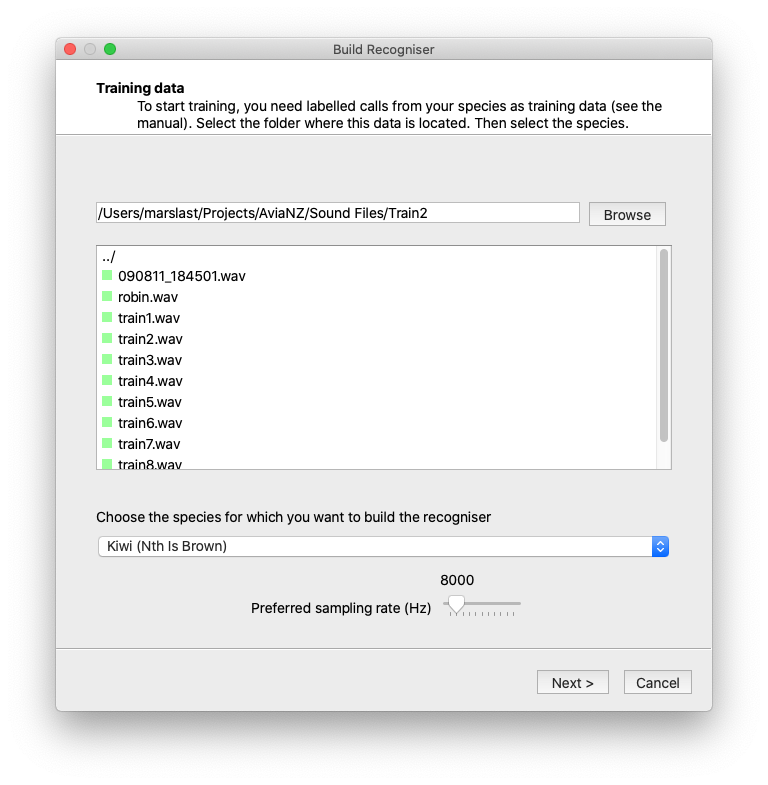
\includegraphics[width=.8\textwidth]{Figures/BuildRecogniser1}
\end{center}

\item AviaNZ will confirm these choices before starting the training process. 
\item There are a few places during the process where you can modify choices that AviaNZ has made. 
\item One is on the first page, where it says `Preferred sampling rate (Hz)'. If you don't know what these things mean, you can ignore them, but for experienced users, there are places where choices that AviaNZ has made might be improved upon.
\item Once the initial choices have been made, press the `Cluster' button, and AviaNZ will try to cluster your labelled training segments into groups of similar sounds (call types, such as male and female kiwi, or `more-pork' and `cree' ruru calls). It will show the outputs of this in this interface:
\begin{center}
    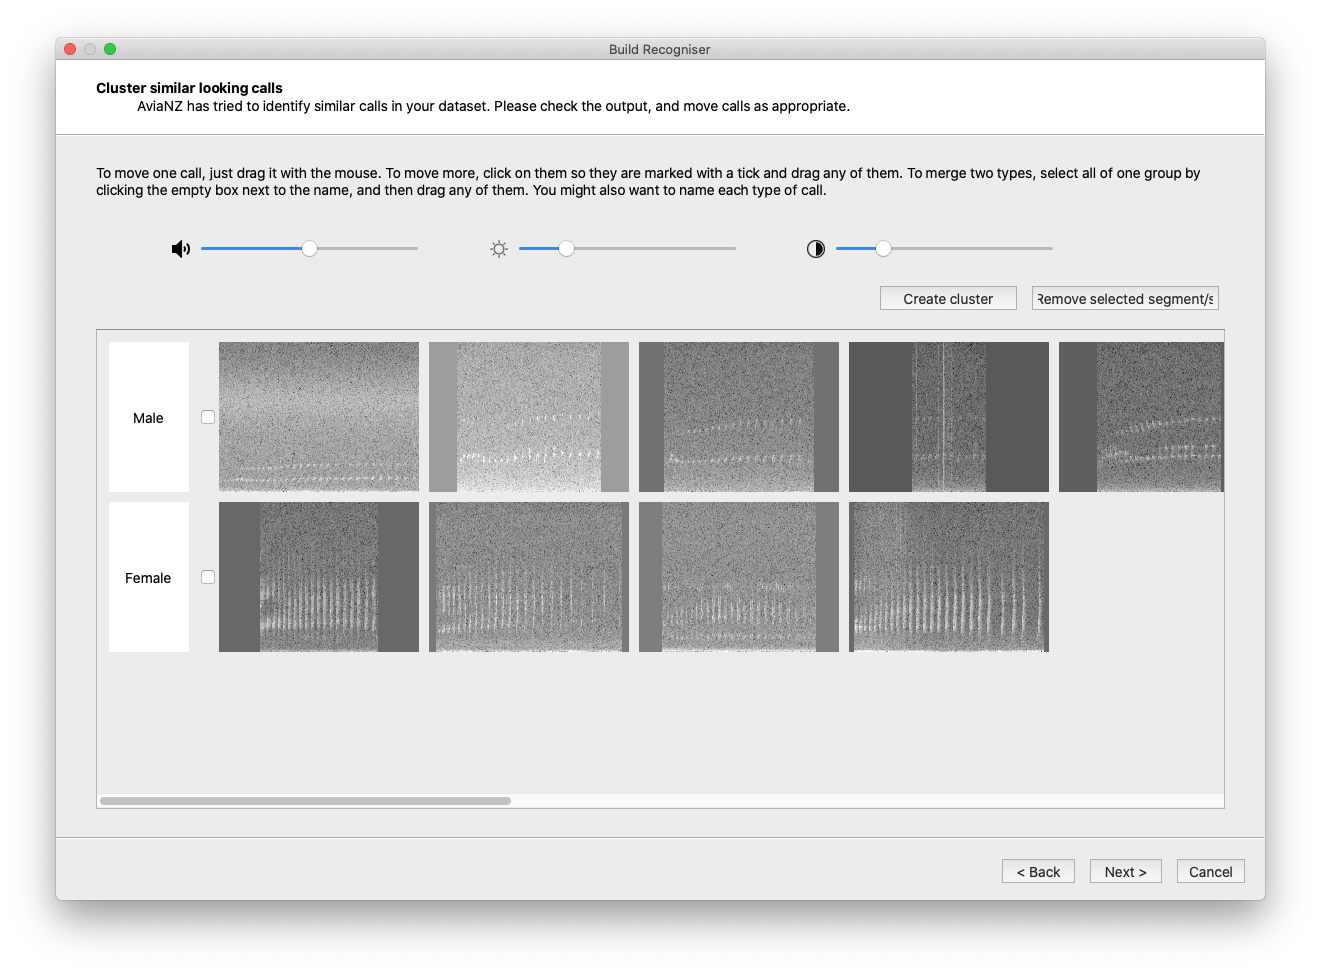
\includegraphics[width=.95\textwidth]{Figures/BuildRecogniser2}
\end{center}
\item We will improve this clustering over time, but at the moment it does make a lot of errors. 
\item There are two ways that you can improve the recogniser that is made:

\begin{description}
\item[Give names to the clusters] It is intended that the clusters each represent different call types or sex of caller for some species. The default names are meaningless, since AviaNZ doesn't know about the species in advance, so it is normally useful to give a meaningful name by clicking on the name and typing a new one. 

\item[Correct any errors] by moving the spectrograms between different clusters as appropriate. 
\begin{itemize}
\item To move a single spectrogram, just drag it to the correct cluster
\item To move a whole group, click on each one (so it is marked with a tick) and then drag any of them to the correct cluster
\item To move some to a new cluster, click on them, and then click on the `Create cluster' button. 
\item To select all of the calls in a cluster, use the small tick box next to the name of the cluster
\item You can play the calls by clicking on the top-left corner of them.
\end{itemize}
\end{description}


    %\caption{As part of the training process, AviaNZ will show a curve showing how different parameter values trade-off between false positives, and false negatives on the training data. A perfect classifier would be on the top-left of the plot, spotting every call and not labelling any other calls as your species. In practice, if you want to see every example of your species calling, the classifier will also make more mistakes where it labels other calls (or noises) as your species: false positives. This means that you will need to spend more time reviewing the outputs after using the recogniser. Clicking on the curve selects the parameter choices for this call type.}

    
\item AviaNZ will now work through each cluster, and train an individual recogniser for that kind of call. 
\item It will show you a variety of parameter settings:

\begin{center}
    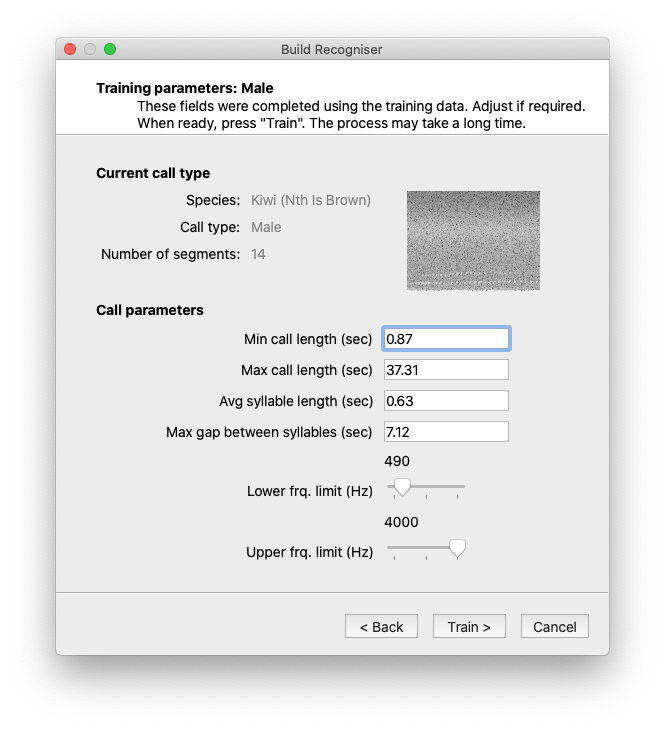
\includegraphics[width=.7\textwidth]{Figures/BuildRecogniser3}
\end{center}

\item If you don't know what they are, just ignore them. 
\item The program will then search for good ways to represent those calls, which can take a while, and then show a plot of error rates for different parameter settings. 
\item This is known as an ROC curve, and it is a plot of the recall (True Positive Rate) against the False Positive Rate for different parameter settings:
\begin{center}
    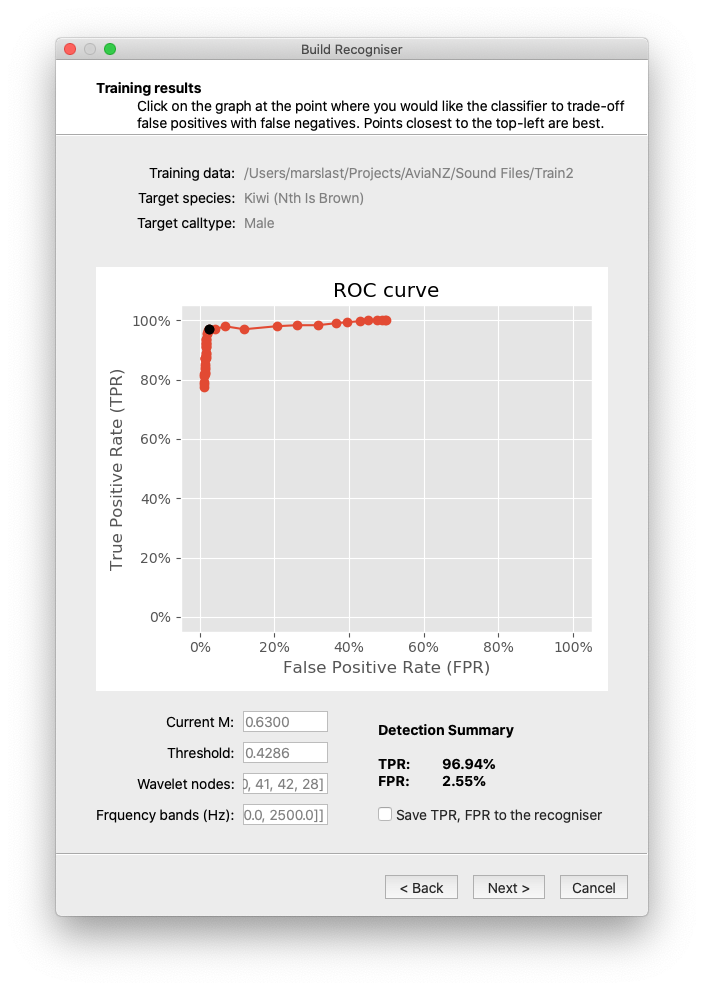
\includegraphics[width=.7\textwidth]{Figures/BuildRecogniser4a}
\end{center}

\begin{itemize}
\item The perfect recogniser would be in the top-left corner of the graph. 
\item Points lower down miss examples of the bird calling, while calls further to the right provide more false detections, i.e., think the bird is calling when it is not. 
\item You need to choose the compromise between these two that you are prepared to accept: more work in reviewing to get rid of false positives, or accepting that the software has not detected every call. If you are planning to train a neural network filter as well, choose to accept more false detections.
\item To make the choice, click near the point that you think is the best compromise on the curve, which AviaNZ will show as a black dot (you can see it in the picture above). 
\item You don't have to click on it exactly, AviaNZ will show you which point is closest to where you clicked. 
\item You need to do this for each call type. 
\end{itemize}

%\item In the Post-processing window, there is the potential to make another practical choice, which is whether or not to use the Fundamental Frequency calculation as part of the filter:

%\begin{center}
    %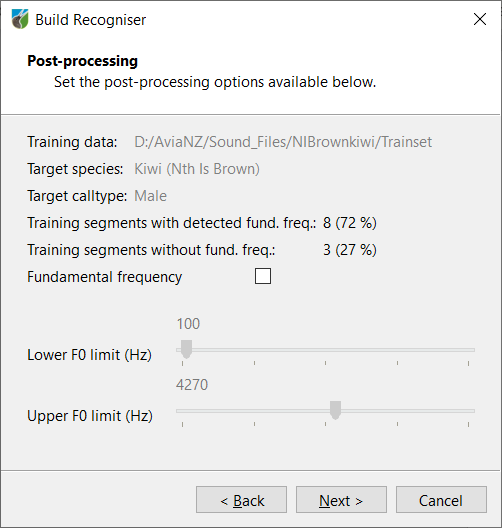
\includegraphics[width=.4\textwidth]{Figs/Wizard_post}
%\end{center}

%\begin{itemize}
%\item For some calls, birds can produce a base note and then harmonics above that, and the fundamental frequency calculation tries to find the base note. 
%\item Where this works it can be helpful, so if you compare the number of training segments where the software found a fundamental frequency with those where it didn't, you can see whether or not it makes sense to use it. 
%\item You can also see the range of frequencies that were identified, so if they look wrong, don't use it. 
%\item If you don't know, AviaNZ will try to work it out for itself. 
%\end{itemize}

\item Following this, you choose a name to save the recogniser you have trained. It is then a very good idea to test it. 
\end{itemize}

\subsection{Extending a recogniser with CNN}\label{sec:cnnfilter}

A wavelet recogniser will usually find most of your bird calls (it has good recall), but the price you pay for this is that it finds a lot of false positives (poor specificity). This leads to a lot of wrong segments that have to be reviewed. You can extend the filter in AviaNZ using a neural network known as a CNN (convolutional neural network). These are often used for image recognition. Training a neural network requires a lot of training data and computational power. The way that you perform the training is as follows:

\begin{description}
\item[Preparation] You will need to compile a good collection of the calls of your species. 
\begin{itemize}
\item Make a new folder, select and copy some field recordings into this folder. The selected recordings should represent the real nature of field recordings that you are going to process with this recogniser, e.g., consider various background noise, call variations etc. If you have multiple recorders and sites, try and use examples from all of them. The more data you have here, the better. We have typically used enough data to have hundreds of examples of each call type.
\item Once you have this data use the `Batch Process' option to apply the trained wavelet recogniser to the set of files. This will likely find the vast majority of the calls, but also a lot of false positives. It may also miss parts of calls, or make the calls too long. 
\item You now need to review these calls. We use a two-stage process for this.
    \begin{description} 
    \item[Remove false positives] Using either of the batch review options, delete any segments that do not contain your target bird call. 
    \item[Correct the segments] Using manual mode, correct the size and location of each segment box so that it covers the call, but only the call. Also check that the call type was labelled correctly and correct any errors. You can swap between seeing the species label and the call type label using the 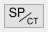
\includegraphics[scale=0.5]{Figures/SPCT} button on the right of the Controls panel. You can also do this second part in the All Species Batch Review (Section~\ref{sec:batchAll}).

    Once you are sure that each label is correct, use the `Confirm labels' (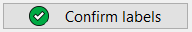
\includegraphics[scale=0.5]{Figures/confirmlabels}) button so that the segment turns green. Or at the end of manual correction of the box sizes, you can review the folder in Batch Review and confirm them to make it faster.
    \end{description}
\item In addition to the batch reviewed recordings, you can also input manually annotated recordings to the CNN training, such as the training data set that you used for the wavelet recogniser training. If you plan to use some other manually annotated recordings (not the train data in wavelet training), make sure to annotate it to include both species and call type. You can use 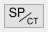
\includegraphics[scale=0.5]{Figures/SPCT} button from the Controls area in the Manual Interface to assign call types. Alternatively, you can annotate the calls to the species level and assign the call type during the review of the folder in the Batch Review All Species review (Section~\ref{sec:batchAll}).
\end{itemize}
\end{description}
 
\begin{description}
\item[Training] Follow the steps below to train your CNN:
\begin{itemize}
\item Select `Train an automated recogniser' $\rightarrow$ `Extend a wavelet recogniser with CNN' from the Recognisers menu. 
\item Follow the instructions to select the folder/s with training data. Use the appropriate `Browse' buttons to load your manually annotated recordings and the Batch Processed and Reviewed recordings. Select the the name of the wavelet recogniser that you will be extending from the list. 

\begin{center}
    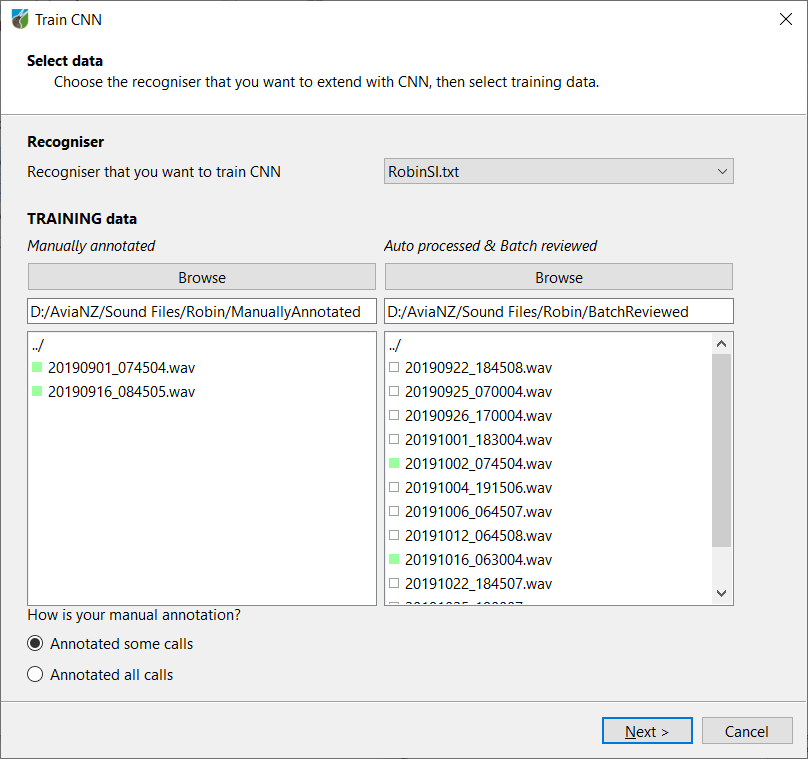
\includegraphics[width=.7\textwidth]{Figures/CNNpage1}
\end{center}

\item AviaNZ will confirm these choices before starting the training process. It will also warn you if it cannot find enough data. 
\item AviaNZ will then suggest an appropriate length of call/segment to feed into the CNN. If the number looks wrong for your species, you can correct it. Ideally this length should be a bit longer than both a syllable of the call, and the gap between syllables. 
\item At the end of the training, AviaNZ will show you ROC curves for each call type and ask you to select a point that represents your compromise between True Positive Rate and False Positive Rate. If you select the relevant option then AviaNZ can do this automatically instead.

\begin{center}
    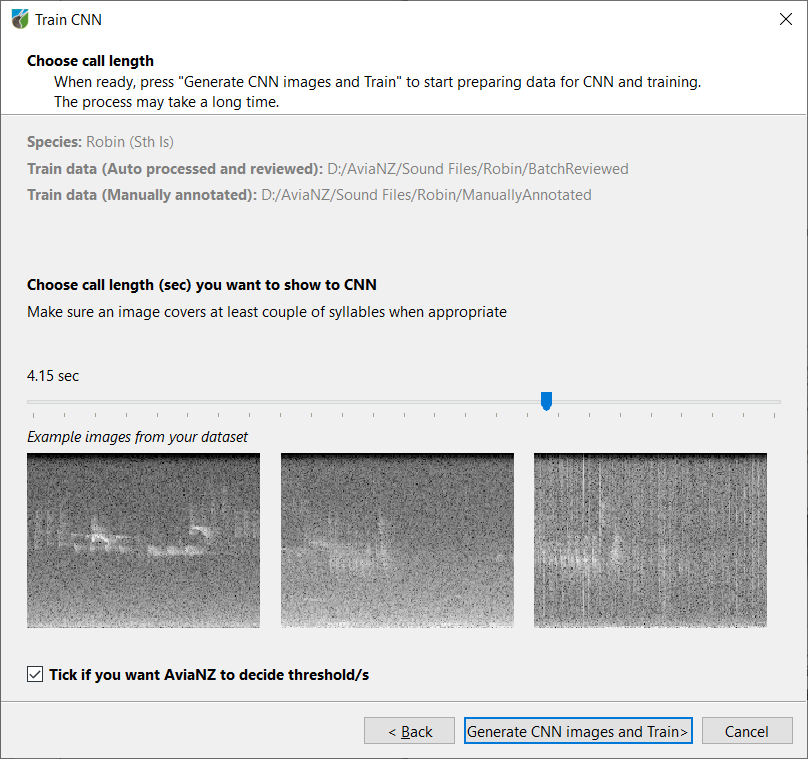
\includegraphics[width=.7\textwidth]{Figures/CNNpage2}
\end{center}

\item It normally takes a long time to train the neural network. 
\item Following training, AviaNZ will show you a summary of the CNN recogniser, and you can choose to save it either as a new recogniser, or updating an old one. This means that you can train multiple recognisers for a species to see which works best. 
\item It is important to test your recogniser on some different data. If the results are not good enough, you will need to rerun the process with more training data and make sure that your labels are good.
\end{itemize}
\end{description}

\subsection{Testing a recogniser}\label{sec:testfilter}

\begin{itemize}
\item You should always test a recogniser, and use different files than the ones you trained it on.
\item If you have prepared testing data already, you can do this straight away. 
\item Otherwise save the recogniser and then test at a later date by using `Test a recogniser' in the Recognisers menu of the Manual interface.
\item You should also test a recogniser that you receive from somebody else (for example, from our webpage) before relying on it.
\item It runs the recogniser over the files, and compares the results to the human annotations using the same error metrics that were defined in Section~\ref{sec:metrics}. It gives a better indication of how well the recogniser will work in practice. %If you look at the testing files after using this feature in the `Manual Processing' interface, you can see the annotations from both the human and machine in order to compare them. 
\end{itemize}



\end{document}
